\subsection{Front tool plate} %Ande

Different prototypes were designed to select one final improved design of the front tool plate. The idea was to make a simple design which would meet all the requirements and at the same time possible and easy to mill. The requirement was to make room for four headlight LEDs, two torpedoes and one sonar. The design should be modifiable and at the same time easy to mill.

Naiad needed to be submersible and the first front tool plate was redesigned and manufactured to make Naiad submersible for the tests. Since this part was temporary and only needed for the tests, it had to be manufactured with a low cost. Therefore, this part was divided into eight parts to make it possible to use free waste materials. See fig. \ref{ToolPlate1} below for the first version of the front tool plate.

All parts where glued together and painted to make it waterproof. The design is simple, there are eight empty spaces inside the front tool plate which can be used to balance out the weight of Naiad and make it submersible.

	\begin{figure}[!ht]
	\begin{center}
		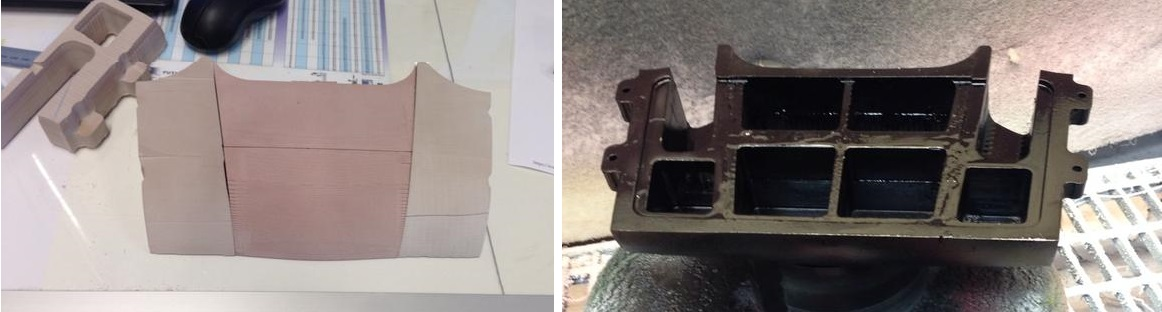
\includegraphics[width=150mm]{./Images/Mechanics/ftp1}
		\caption{The first version of front tool plate which made Naiad submersible for the tests.}
		\label{ToolPlate1}
	\end{center}
\end{figure}

The second version of front tool plate was manufactured by milling as one big part and it is made out of plastic. The plastic has a good heat resistance, the impact strength is high, it is high resistance to abrasion and it has 1.25 g/cc density which is much heavier than water \cite{ftpplastic}.

	\begin{figure}[!ht]
		\begin{center}
			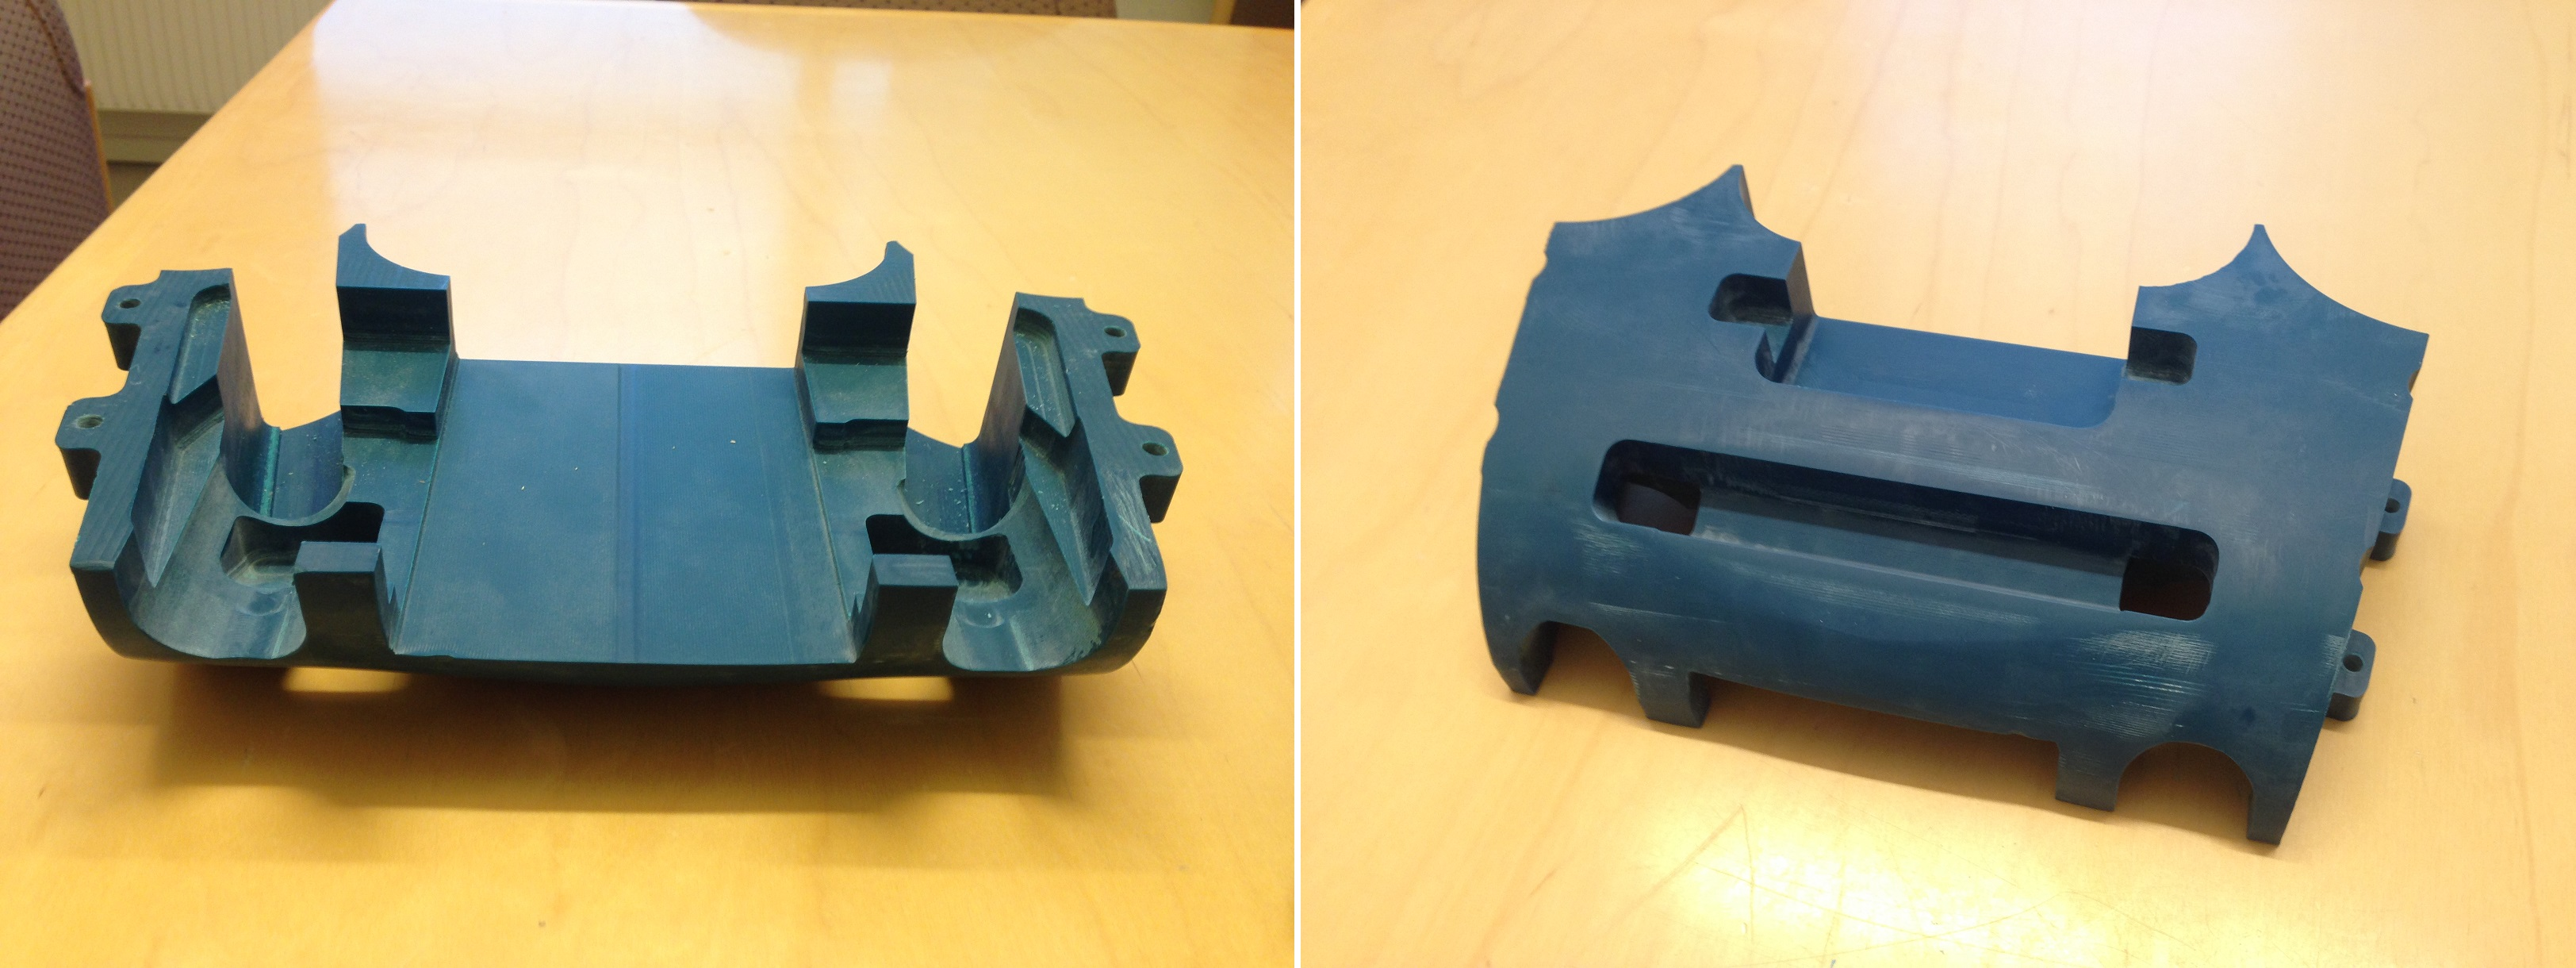
\includegraphics[width=130mm]{./Images/Mechanics/ftpplastic.jpg}
			\caption{The second manufactured front tool plate.}
			\label{plastic}
		\end{center}
	\end{figure}

Naiad needed headlights for both cameras, the one facing forward and the one facing to the bottom. In the beginning it was planned and designed so that the headlight for the front camera should be placed in the main hull. However, the LEDs used for headlights easily became very hot and therefore needed a cooling system. This was difficult to provide inside the main hull where all the electronic are placed, so the headlights were moved to be placed in the front tool plate instead which was the only place for headlight which could provide them a cooling system and was close to both of the vision systems at the same time.

	\begin{figure}[!ht]
		\begin{center}
			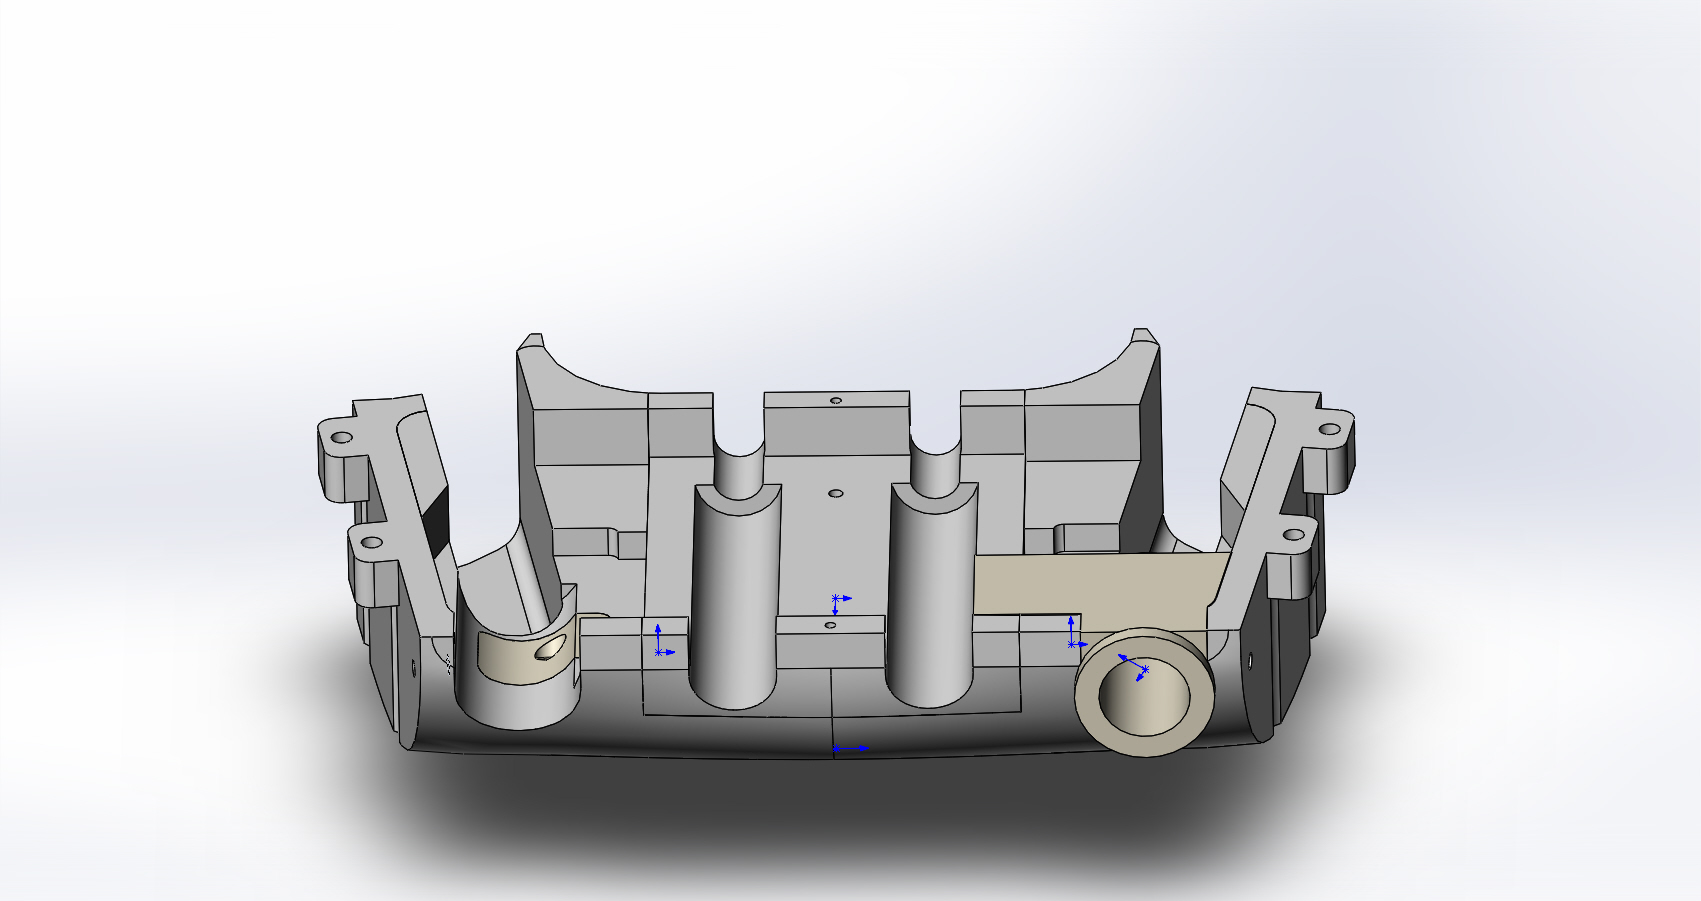
\includegraphics[width=120mm]{./Images/Mechanics/FTPv7leds.JPG}
			\caption{Front tool plate with right highlightbox}
			\label{rightlight}
		\end{center}
	\end{figure}


Two headhlight boxes will be placed on each side of front tool plate, see the fig. \ref{rightlight}, and one box with two LEDs inside will be attached to the bottom of front tool plate, fig. \ref{bottomleds}.


There are two cables coming out from the main hull that have to go through the front tool plate and out to the thrusters. This is why there is an empty space on each side on the back of the front tool plate which gives a free passage to the cables, see fig. \ref{tcablespace}.

	\begin{figure}[!ht]
		\begin{center}
			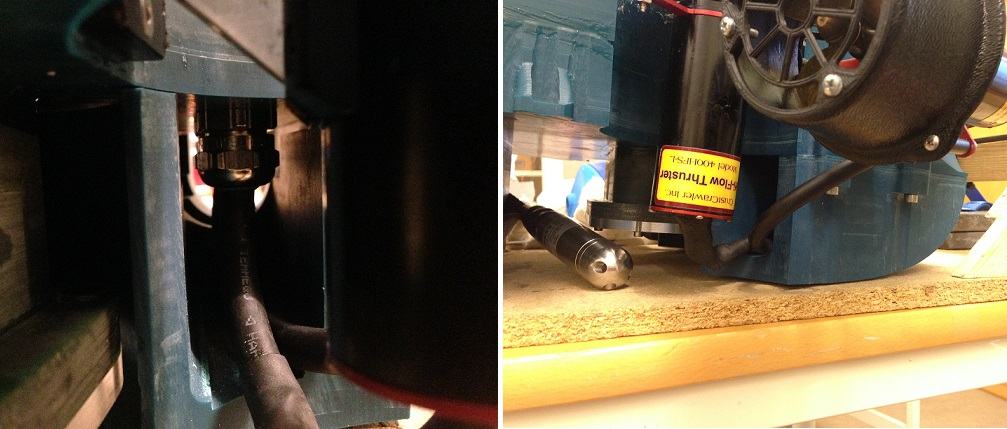
\includegraphics[width=150mm]{./Images/Mechanics/tcablespace.jpg}
			\caption{Front tool plate with right highlightbox}
			\label{tcablespace}
		\end{center}
	\end{figure}

The problem with the design was that it was difficult to make room for all the equipment, to fulfill all the equipment requirements and to make it easy at the same time to mill.

Since a sonar will be used to scan the front and the bottom it had to be placed in the front of the front tool plate. To make it possible to scan both front and bottom the sonar needed to be placed with a 25 degree angel facing down. 

The requirement for the sonar made it impossible to mill the front tool plate, the 25 degree angel was impossible to mill. The solution was to make a sonar box and by screws attach it to the front tool plate.
The box would also make the sonar changeable in case the sonar would not be needed or needed an upgrade. More information about the sonar box can be found in section \ref{sonarsection}.

To make it possible to screw the sonar box to the front tool plate two plugs were designed, milled and glued to the front tool plate, fig. \ref{plug}. The plugs were made since they had a 25 degree, like the sonar box, which was impossible to mill together with the front tool plate as one whole part. One of the plugs is designed to give path to the cables which comes out from the sonar box. The cable from the sonar box will come out through the empty space behind the front headlights and go in through the tool plate into the main hull. All the cables can go the same way into the main hull. However, depending on which system is used to fire torpedoes a different path can be used. There is an empty space around the cameras which makes it possible for wires to go through into the tool plate.


	\begin{figure}[!ht]
		\begin{center}
			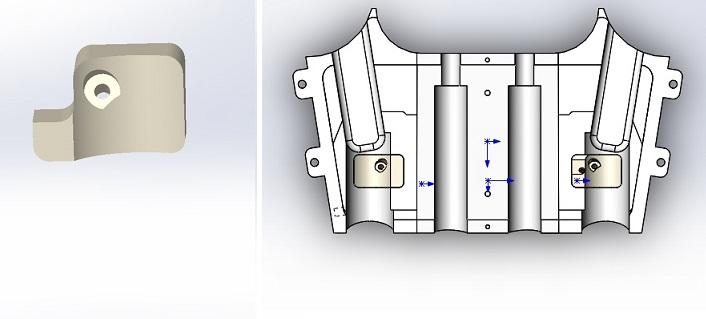
\includegraphics[width=150mm]{./Images/Mechanics/ftplug.jpg}
			\caption{The first picture shows the plug and the second shows where the plugs are glued}
			\label{plug}
		\end{center}
	\end{figure}
	
One of the Robosub requirements is to have a torpedo launcher which should fire at a target in the competition. Naiad will have two torpedoes placed in the middle of the front tool plate close to the front camera system, more information about how the torpedoes works can be found in section \ref{torpedosection}.

	\subsubsection{Headlights}

It was a challenge to make a good design of the headlight boxes. The design needed to fulfill the requirements and at the same time be easy to manufacture. The basic idea of the headlight boxes is to make it easy to change the LEDs in the future, but the most important was to provide it with a cooling system. The design is simple, a plexi glass is attached by screws to the front of the box which are waterproofed by an O-ring in between. The glass is then easily removable which makes the LEDs changeable.

The headlight box could be manufactured in two different ways. If it is made in plastic then the bottom,  which the LEDs will be attach to, should be made by aluminum. The other idea is to make the whole box made by aluminum, which will cost more but is much more effective of reducing the heat. 

Each of the front boxes was divided into two parts, milled separately and glued together to one whole part. 

The cooling system for the bottom box is simply that the whole box is made by aluminum and the empty space between the box and the front tool plate will provide a water flow around the box. 
The cooling system for the front boxes are much more simple, it is based on the same idea that the whole boxes are made by aluminum and there is an empty space behind which provides a water flow.


	\begin{figure}[!ht]
		\begin{center}
			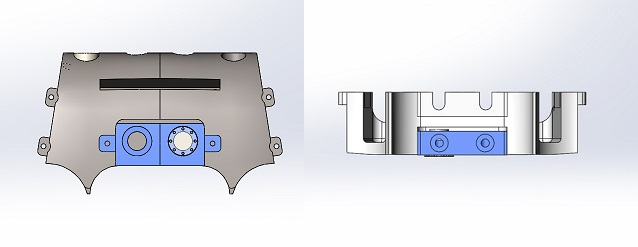
\includegraphics[width=150mm]{./Images/Mechanics/Ledb.jpg}
			\caption{Bottom highlight box}
			\label{bottomleds}
		\end{center}
	\end{figure}

	\subsubsection{Sonar} 
\label{sonarsection}
Many different prototypes were made to make it possible to mill. The final solution was a box with a 90 degree angel in one side and a 115 degree in the other the side. On each side of the boxes there is one hole for the screws and one side has one more hole for the sonar cable. The box was milled and sent to DeepVision to attach the sonar to it and to make it waterproof.

	%\begin{figure}[!ht]
	%\begin{center}
	%	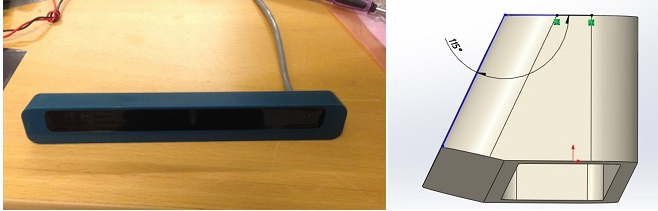
\includegraphics[width=150mm]{./Images/Mechanics/sonar.jpg}
	%	\caption{The sonar box, picture one shows sonar attached to the box.}
	%	\label{sonar}
	%\end{center}
%\end{figure}

	%\begin{figure}[!ht]
	%\begin{center}
	%	\includegraphics[width=100mm]{./Images/Mechanics/FTPsonar.JPG}
	%	\caption{Shows where the sonar box are attached.}
	%	\label{sonar2}
	%\end{center}
%\end{figure}

	\label{sonar}
	\subsubsection{Torpedoes}
Since torpedoes was only required for the RoboSub competition and may not be needed in the future use, the design of both the front tool plate and torpedo launcher should be modifiable. Therefore a torpedo launcher box was designed and a part of it was manufactured. The torpedo launcher will be attached to the box and the box will be attached by screws to the front tool plate. 


	\begin{figure}[!ht]
		\begin{center}
			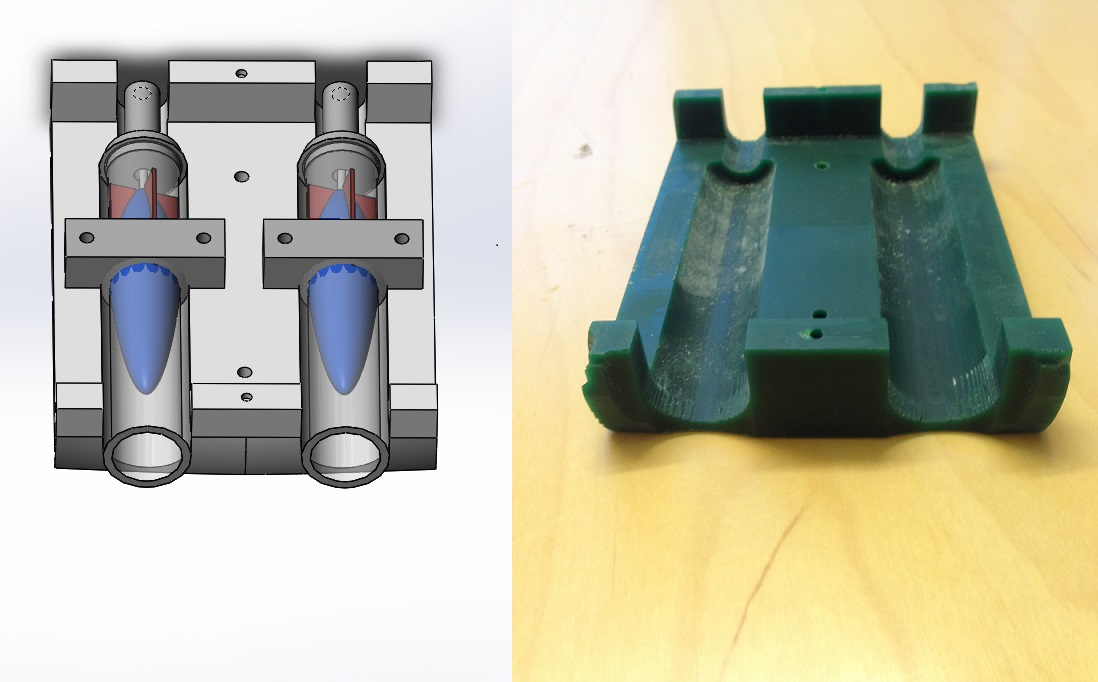
\includegraphics[width=100mm]{./Images/Mechanics/tplh.jpg}
			\caption{The torpedo launcher box.}
			\label{torpbox}
		\end{center}
	\end{figure}

The torpedo box is also made by the free waste material and the box is a prototype for using the pneumatic system torpedo launcher, see fig. \ref{torpbox}.


	\label{torpedo}
